\documentclass{llncs}
\usepackage{tabularx,colortbl}
\usepackage[dvipsnames]{xcolor}
\usepackage{flushend}
\usepackage{cite}
\usepackage{amsmath}
\usepackage{amssymb}
\usepackage{epsfig}
\usepackage{stmaryrd}
\usepackage{url}
\usepackage{multirow}
\usepackage{latexsym}
%\usepackage{float}
\usepackage{graphics}
\usepackage{graphicx}
\usepackage{enumitem}
\usepackage{comment}
\usepackage{longtable}
\usepackage{supertabular}
\usepackage{caption}
\DeclareCaptionType{copyrightbox}
\usepackage{times}
\usepackage{listings}
\usepackage{subfigure}
\usepackage{color}
\usepackage{balance}
%\usepackage{clrscode3e}

\gdef\SetFigFont#1#2#3#4#5{}

\captionsetup{font=normalsize,labelfont=normalsize}
\usepackage{algorithm}
\RequirePackage[noend]{algorithmic}
\renewenvironment{algorithm}[1][\textwidth]%
{\begin{minipage}[t][\totalheight][c]{#1}\begin{algorithmic}[1]}  %%% change [1] to [0] to turn off line numbers
{\end{algorithmic}\end{minipage}}

%\definecolor{nsrcolor}{rgb}{0.7,0.0,1.0}
%\newcommand*{\nsr}[1]{}%{\textcolor{nsrcolor}{\noindent\textbf{[nsr:~}\textit{#1}]}}

%% %% Use for each in ``FOR'' constructs
\renewcommand{\algorithmicfor}{\textbf{for each}}

%% %% All comments are in italics
\renewcommand{\algorithmiccomment}[1]{\textit{${/\ast}$~#1~${\ast/}$}}

%% %% Use ``procedure'' instead of ``Algorithm'' for off set
\renewcommand{\algorithmicensure}{\textbf{procedure}}

\newcommand{\algoname}[1]{\ENSURE #1}
\newcommand*{\algobox}[1]{\framebox{#1}}


\definecolor{lightgray}{gray}{0.9}

%\usepackage{hyperref}

\newcommand{\tab}{\hspace*{3ex}}
\newcommand{\codetab}{\hspace*{2ex}}
\newcommand{\tinytab}{\hspace*{.75ex}}

%% Create a uniform and easy to change reference to figures and tables.
\newcommand{\figref}[1]{Fig.~\ref{#1}}
\newcommand{\tabref}[1]{Table~\ref{#1}}
\newcommand{\eqnref}[1]{Eq.~(\ref{#1})}
\newcommand{\secref}[1]{Section~\ref{#1}}
\newcommand{\defref}[1]{Definition~\ref{#1}}


\begin{document}
\newcommand{\mcdc}{}%MC/DC}
\newcommand{\mike}[1]{\textcolor{red}{Mike: #1}}
\newcommand{\anitha}[1]{\textcolor{red}{#1}}
\newcommand{\oksana}[1]{\textcolor{magenta}{Oksana: #1}}
\newcommand{\sjp}[1]{\textcolor{blue}{#1}}
\newcommand{\nsr}[1]{\textcolor{blue}{#1}}
\sloppypar


\title{From Informal System Requirements to Formal Software Specifications  - An Experience Report\thanks{This work has been partially supported by NSF grants CNS-0931931 and CNS-1035715.}}

\author{Anitha Murugesan, Daniel A. Cofer, Michael W. Whalen, and Mats P.E. Heimdahl}
\institute{Department of Computer Science and Engineering,\\
 University of Minnesota, 200 Union Street, Minneapolis, MN 55455,USA\\
\email{\{muru0011,cofer008, whal0046, heimd002\}@umn.edu}
}

\maketitle

\begin{abstract}
Formal methods have been enormously useful in verifying complex system requirements. However, their success depends on precisely formalizing {\em what} needs to be verified and thoroughly understanding {\em how} it is verified. While the advances in formal methods has given rise to sophisticated techniques and tools, there is a lack of awareness and methodological guidance in using these techniques effectively, that often makes their use difficult and the results of their application leading to overconfidence in the correctness of the fielded system in its intended environment.

In this paper, we report on using formal methods to verify a complex infusion pump system.  While the effort was successful and has led to end-to-end verification of a hierarchically composed software architecture, it was not without challenges that we believe are not adequately presented in the research literature. In our experience, we found that (a) precisely identifying the contextual information for requirements when formalizing them from traditionally structured requirements document is a non-trivial task, (b) some incorrect guidance exists on ``flowing down'' system requirements to lower levels of abstraction that could cause misinformed judgement about the correctness of the system, (c) inadequacy in understanding the technicalities of the formal tool can lead to ``proofs" based on faulty premises, and (d) inadequate mitigation of risks when using multiple analysis tools can result in misplaced confidence about the system. We then explain our approach to identify, mitigate and address such concerns.

\end{abstract}

\section{Introduction}
\label{sec:intro}

%Complex cyber-physical systems are often developed hierarchically through decomposition of a ``top level'' system into layers of smaller and more manageable components.  Decomposition is performed to accommodate reuse, integration with existing or commercially developed components, and distributed development, as well as to factor the complexity of development~\cite{Hammond01:WiW}, and the process of decomposition typically involves identifying  components and their interconnections as well as allocating requirements to each of them. One of the challenging tasks in this process is determining \emph{``if the composition of component behaviours satisfy the overall system requirements?''}.

In safety critical systems, formal methods (mathematical techniques) are often used to rigorously assure the correctness of systems. %However, the challenge in successfully using formal methods lies in precisely stating ``what" needs to be verified and thoroughly understanding ``how" it is verified, rather than the action of verification itself.
While advances in technology has improved the verification capability and efficiency of formal tools such as model checkers, they still rely on the skill level of the engineers to correctly formalize requirements
and understand the technicalities of the tools. For instance, one could use a set of inconsistently (or incorrectly restrictive) formalized premises to prove requirements using formal tools and gain misplaced confidence about the successful but meaningless verification. While there are numerous success stories that illustrate the benefits of using formal methods~\cite{Miller03:shalls,Whalen07:FMICS} as well as discussions about the limitations of formal methods~\cite{kneuper1997limits,hall1990seven}, we believe that % there are aspects of application of formal methods that remain necessary to discuss.
there are not adequate discussions about the practical challenges encountered and techniques adopted to mitigate them in real applications.
In our opinion, codifying the pitfalls will allow wider and better dissemination of formal methods in industrial use.

In previous work~\cite{hilt2013, req2code, ICCPS2014}, we proposed scalable and efficient model based approaches to verify the formalized requirements of complex control systems, given their architecture (hierarchical decomposition into components) and formalized requirements. The approach involved hierarchically modeling, formalizing and verifying the requirements of the system and its components using multiple tools% (Simulink, Simulink Design Verifier~\cite{SimulinkDesignVerifier} and AADL/AGREE~\cite{NFM2012:CoGaMiWhLaLu})
, each with slightly different formal representations and usage. While this approach was useful to verify hierarchically decomposed systems, when we used it to verify an substantially complex medical infusion pump system, we faced a number of practical challenges and pitfalls that had the potential to undermine the value of not just our approach but formal requirements analysis in general. %These challenges, that lie in the intersection of the requirements engineering and formal methods domains, are aspects of application of formal methods remain necessary to discuss in-spite of their wide spread use. %have not been discussed in depth and addressed in any existing literature.

In this paper we discuss the challenges we faced while formally verifying requirements at multiple levels of hierarchy, applying tools and techniques ``at scale'' involving several developers over an extended period of time.  We focus on four challenges:
\vspace{-0.15in}
\paragraph{\textbf{Requirements Formalization:}} Identifying the contextual information when formalizing requirements from a traditionally structured requirements document is a challenging task. In our effort to formalize the requirements of an infusion pump, we spent an enormous amount of time to identify the context for each requirement, even though the requirements were organized as per standard templates~\cite{IEEESRS}. This is mainly because the way of the requirement statements are linearly organized within the document did not help precisely identify its context. To overcome this challenge, we hierarchically organized the requirements within the document that not only clarified the context for each requirement while formalizing them but also improved the clarity of the document.
\vspace{-0.15in}
\paragraph{\textbf{Requirements Refinement:}} When systems are decomposed and requirements are allocated to its components, establishing the fidelity between the system and its component requirements is a challenge, especially when system requirements are informally expressed and component requirements are formally specified. While decomposing the infusion pump system, we derived formal software requirements from the natural language system requirements using an approach proposed by Miller et.al~\cite{Miller01:dasc} (also used in other papers such as~\cite{jeffords2010model,kauppinen2007re, lempia2009requirements}), but found that it led to incorrect compositions when we tried to establish system requirements. %The approach does not consider the inherent relational aspect of system requirements and the functional aspect of  requirements of components like software, that lead to incorrect requirements allocation. 
To address this concern, we propose documenting a \emph{satisfaction argument}, originally described by Jackson~\cite{jackson1995world}, that captures the relationship between the system and component requirements as well the assumptions that are necessary to establish that relationship. Explicitly documenting this argument for every requirement allowed us to validate both the requirements allocated to the components and the related assumptions.
\vspace{-0.15in}
\paragraph{\textbf{Cursory Knowledge of Tools:}} In an hierarchical architectural proof approach, all proofs are predicated on ``leaf level'' components meeting their requirements. If these leaf-level requirements are incorrect (infeasible or inconsistent), then the proof is not well-founded. While formalizing the leaf level component requirements for the infusion pump, we unknowingly formalized some computations used within requirements in a inconsistent and unrealizable way, that was not detected by the tools and lead to misplaced confidence about the system. This prompted us to request for changes and enhancements to the tool to check {\em realizability}~\cite{gacek2015towards} and {\em consistency} of requirements.
\vspace{-0.15in}
\paragraph{\textbf{Matching Tool Boundaries:}} In order to be able to reason at scale about complex systems, we found it necessary to use multiple reasoning tools at different levels of abstraction within the software architecture. This use necessitated translation of properties between multiple tools. However, the mere action of transcription of requirements between different notations of the tools (even through the tools shared the “same” semantics) induced several errors that lead to misplaced confidence in results. To have adequate confidence in the composition of the results, tools to translate between formalisms were required. 

The contribution of the paper is reporting the challenges and non-obvious nuances in using formal methods to verify requirements of complex systems that, we believe, engineers will likely encounter. To some extent, although these limitations seem obvious once stated, in our experience, these issues are not fully realized and mitigated by some parts of the formal requirements analysis community. While we illustrate our lessons learned using the infusion pump we believe many engineers working on similar applications, especially in the safety critical system domain, will face similar challenges and hence we hope that sharing our experience proves instructive.

%is two-fold: first, we report on the successful application of formal methods on a large and complex software architecture (the completion of the work in~\cite{hilt2013}). Second, we
%reporting the challenges in using formal methods to verify requirements of complex systems, that engineers will likely encounter especially in the safety-critical domain, and how we addressed these challenges. %In sum, we assert that the benefits of formal methods in verifying requirements can be misleading, unless there is a change in both requirements engineering activities to support formal methods as well as in formal techniques to recognize requirement engineering concerns. In this paper, we report on the challenges and non-obvious nuances in using formal methods to verify an infusion pump's requirements. We also describe our approach to overcome those challenges from both requirements engineering and formal methods perspective.
%While we illustrate these lessons learned using the infusion pump we believe many engineers working on similar applications, especially in the safety critical system domain, will face similar challenges and hence we hope that sharing our experience proves instructive. %The intent of this paper is to serve as as lessons learnt and best practices for practitioners and researchers involved in similar efforts.

The paper is organized as follows. In Section \ref{sec:gpca-overview} we provide a brief overview of our previous effort that serves as a context for the issues described later. In Section \ref{sec:challenge} we explain the specific challenges and pitfalls we encountered while verifying the infusion pump system along with our approaches and recommendations to address them. Finally, we conclude the paper in Section \ref{sec:conclusion}.
\iffalse

%
%applying hierarchical reasoning amongst a team of developers over time on a complex system architecture.
%
%constructing models, determining requirements for different levels within the hierarchical description (e.g., describing top-level software vs. system requirements), and correctly formalising English-language requirements.  It extends the work in~\cite{hilt2013}, as we have scaled up this description to a much more substantial model.
%
%The approach was based on the presumption that the we correctly formalized the requirements of both system and components and understood how the tools worked; unfortunately that was not an easy task.
%
%be formalized using a variant of temporal logic, that was unfortunately a challenging task. Further, .
%%required us to we faced a number of challenges in the process of precisely formalizing and verifying the requirements, the
%% and deriving component requirements from the natural language system requirements as well as ensuring if they are accurately verified.


\anitha{I would like to explain the 4 challenges in the introduction. But it has become 4 long paragraphs.}
%
In particular, we focus on four challenges that we believe have not been discussed in depth in existing literature. First of all, systematically identifying dependencies between requirements while formalizing them from a traditionally structured requirements document is challenging. Typically, system requirements are captured using natural language and organized as per one of existing requirements document templates~\cite{IEEE formats}. However, we found that this traditional structuring of the requirements makes the task of formalizing requirements arduous and error prone. \mike{What does this mean?  Dependencies in what sense?  I don't understand this paragraph}


%, and our approach to address them Hence, we restructured the infusion pump requirements in an unique way that made it conceptually easy to understand and formalize.

Secondly, we found that understanding the mathematical differences between formalized system and component requirements is crucial, since it may otherwise lead to inaccurate analysis of the system. While decomposing the system and allocating requirements to components, especially the software of the system, it has been a practice~\cite{extending4variabe} to replicate the system requirements into software requirements by just changing the scope. However, while formalizing the requirements for the infusion pump software, we found that most system's requirements were typically expressed to account for tolerances, whereas the corresponding software requirements did not need such allowances. In mathematical terms, the former was relational whereas the latter was functional. We realized that failing to recognize such mathematical differences between the requirements may result in incorrect assurance of the system. %To identify such errors, we used a richer traceability document for the infusion pump.

\anitha{Should i mention which tool we use here?}
Thirdly, we posit that cursory knowledge about how the formal tools perform  verification can lead to highly believable but erroneous results. While verifying the requirements of the infusion pump, we found that the tool successfully verified requirements that were inconsistently formalized. While the tool was sophisticated enough to detect such issues, it could do so only if certain options were explicitly set in the tool's configuration; that, unfortunately, was not obvious. Although the root cause of the `cursory knowledge' was due to the limited information provided by the tool about such options along with the verification results, this ultimately resulted in successful proofs of inconsistent requirements.

Finally, we also found that when recapturing verification results from one tool to another, even if their notations have the ``same" semantics, the mere transcription of requirements from one notation to the other may lead to elusive errors. To verify the infusion pump system we used two tools in a successive fashion such that the verification results from one tool will be used by the other. Although the notation used in both the tools to formalise requirements were semantically same, the mere action of recapturing the requirements between the tools resulted in transcription errors that were difficult to detect.

By ``cursory knowledge'', we mean the engineer's knowledge about all the default or normal configuration of the verification tool, that are often hidden. does not make it explicit, it may be unreasonable to expect the engineers to have in-depth tool knowledge,   %Such options are usually intensionally disabled by default to improve the tools performance. Hence, it relies on the expertise and knowledge of the engineer to recognize the need for such options. When we found such issues with the help our tool expert, we requested the tool developers to make such configuration information obvious to users.

Given the architectural model of the system and formalized requirements (both system and the components), we used tool called AGREE (Assume Guarantee Reasoning Environment) to automatically verify if the decomposed component requirements are sufficient to guarantee the system level requirements. Subsequently, we also verified if the component requirements are indeed satisfiable by each of their respective implementations (modeled using Simulink/Stateflow tool), using MathWorks Simulink Design verifier (SDV) tool. This tool chain allowed us to rigorously verify the decomposition of the infusion pump requirements in a scalable and efficient manner. However, the process of precisely formalizing requirements and deriving component requirements from the natural language system requirements was a non-trivial activity. In the following sections, we elaborate on the challenges  and our approaches we address them.
The intent of this paper is to serve as a report of practical challenges and lessons learnt while using formal methods to engineer requirements of safety critical systems from a practitioner's perspective.

Infusion pumps have been involved in many incidents, posing hazards to patients, due to their malfunction. To contribute to The US Food and Drug Administration's (FDA)~\cite{fda2010whitepaper} initiative to improve the safe development of these devices, we demonstrated an end-to-end model based approach to develop high assurance infusion pumps using a generic infusion pump system.

The overall system requirements especially for complex control systems such as GPCA are typically captured to accommodate certain degree of inaccuracies and imperfections in the environment, that interacts with the system, and the physical components, that would be used to construct the system. But, when the GPCA was decomposed and requirements were allocated to components the degree of inaccuracies and imperfections in component requirements changes (typically reduces). However, it has been a common perception that most system requirements can trace almost entirely to requirements on one component and hence such system requirements can be recaptured into identical component requirements~\cite{Miller01:dasc}. Unfortunately, in our experience, we found that although some component requirements might seem to be similar to their corresponding system level requirement, a simple recapture of the requirements might be risky. For instance, while GPCA system requirements included tolerances, the GPCA's software did not require such tolerances in their requirements, due to its deterministic behavior. In mathematical terms, while the system requirements were expressed as relations, the software requirements were expressed as functions. Failing to recognize such differences in mathematical notations while formalizing requirements lead to misunderstanding about the decomposition.

Even after precisely capturing the requirements formalizing them for verification from its natural language source was another challenge. We found that operational requirements, that describe the functions performed by a system under normal operating conditions, typically captured using natural language can be easily understood and interpreted. However, when formalizing them for verification it is often the case that it insufficient to just recapture what has been specified in natural language. It is necessary to identify and preclude the exceptional conditions/scenarios that prevent the normal functions from occurring. In the GPCA, to verify if the system infuses drug into patients at a specified rate for a specified amount of time, we had to formalize the requirement in such a way that all the exceptional conditions that will not allow the infusion to occur is excluded. These conditions are usually specified in another requirements but it was a laborious trial and error task to identify them and formalize them appropriately. While one could argue that this is due to imprecisely specified natural language requirements, in practice, these concerns prop up only during formal verification. Although there are numerous case studies that describe success stories of using formal methods to verify requirements, unfortunately none of them elaborate on their approaches and challenges involved in formalizing such requirements.

Further, the results from formal tools could be misleading if one lacks in-depth understanding of how the tools perform verification. One well known problem with formal tools is verifying requirements \emph{vacuously} - in other words successfully verifying a requirement in an unintended (say trivial) manner. Similarly, in our experience we found that it is easy to unknowingly formalize and successfully verify internally inconsistent requirements, if we do not have an indepth understanding of how the specific tool verifies such requirements. While the tools that we used to verify GPCA had the capability to identify such issues, they had to be explicitly enabled in the tool's configuration. Since, such options were intensionally disabled by default to improve the tools performance, it relies on the expertise and knowledge of the engineer to recognize the need for such options. Failing to understand these tool configurations may cause believable but misleading verification results.

While it is well known that there is no "one size fits all" tool/notation to verify requirements especially large and complex ones, bridging the boundaries between different tools to perform system verification is often very problematic. When we use multiple tools and notations to capture and verify requirements, one well known challenge is rigorously bridging the syntactic and semantic differences between them. However we found that, even if they share the "same" semantics, the translation and verification of requirements between tools leads to errors that were difficult to detect.

In practice, the act of formalizing the requirements in a way that is verifiable and decomposing them into component requirements from its natural language source is not an easy task.

(that is also used in other papers such as~\cite{jeffords2010model,kauppinen2007re, lempia2009requirements}),

\fi

\section{Background}
\label{sec:gpca-overview}

In this section, we describe our prior work~\cite{hilt2013, req2code} on modeling and formally verifying the requirements of an infusion pump that forms the basis of this paper. We provide a brief overview of an infusion pump system, its modeling and verification activities that is required to understand the formalization challenges described later in the paper. Infusion pumps are medical cyber physical systems used for controlled delivery of liquid drugs into a patient's body according to a physician's prescription (the set of instructions that governs infusion rates for a medication). Unfortunately, these devices have been involved in many hazardous incidents that triggered the need to strengthen the current system development practices for such systems. Our aim is to demonstrate a rigours model based development approach using a generic infusion pump system that, along with the artifacts we develop in the process, can be be used as a reference for researchers, manufacturers and certification authorities.

\subsection {System Overview}
We considered a Generic Patient Controlled Analgesia Infusion Pump (GPCA), a special type of infusion pump that allows patients to self-administer a controlled amount of additional drug. %Figure~\ref{fig:gpca-overview} shows a GPCA device in a typical usage environment in which a clinician sets up the device and the patient receives the medication from the device through an intravenous needle according to the programmed prescription. To enhance safety of the device it is usually connected to a repository (hospital pharmacy database) that stores manufacturer provided drug limits.
% \begin{figure}[h!]
%    \centering
%    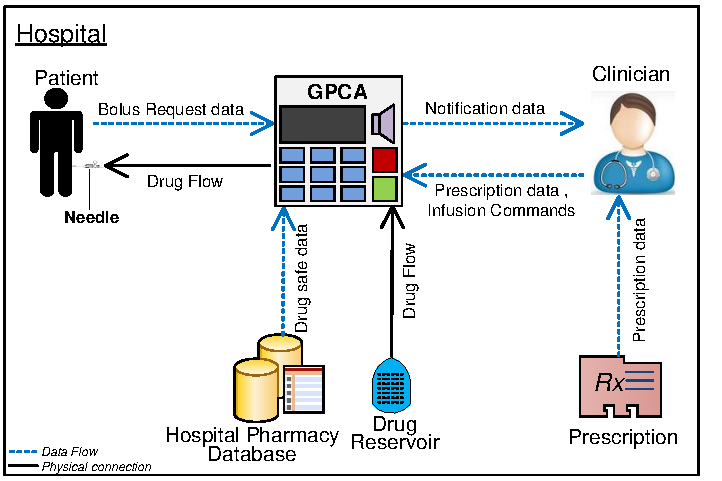
\includegraphics[scale=0.6]{images/Overview.pdf}
%    \caption{GPCA System Overview}
%    \label{fig:gpca-overview}
% \end{figure}
In order to analyse the problems associated with modern infusion pumps available in the market, we considered several advanced capabilities in the GPCA. For instance, we considered three types of infusion options for drug delivery for the GPCA - (a) \emph{basal} infusion in which the drug is delivered at a constant (and usually low) rate for an extended period of
time, (b) \emph{intermittent bolus} infusion that delivers drug at a higher rate for a short duration at prescribed time intervals according to some therapy regimen, and (c) \emph{patient bolus} that delivers additional drug in response to a patient's request for more medication. In addition, we also considered advanced safety features in the device to detect hazardous anomalies/behaviours and mitigate it by notifying the clinician and/or inhibiting infusion and other device operations.

\subsection {System Modeling and Verification}

Our interest with the GPCA is to develop and demonstrate a rigours end-to-end development approach, using model based techniques. We captured a reasonably complete set of overall system requirements using documentation patterns~\cite{mavin2009easy} and standard templates~\cite{IEEEFormats} that we thought will make the task of formalizing requirements straightforward in the verification phases. To cope with the complexity of modeling and verifying the GPCA we followed a hierarchical decomposition approach, that allows the modeling and verification to be systematically and rigorously partitioned into smaller and manageable tasks. In this approach, the system is hierarchically decomposed into a set of interconnected components (its architecture) and each component is allocated with its own set of requirements. At the leaf level, in addition to the allocated requirements, the detailed behaviour of each component is captured. This approach allows us to establish the requirements of the overall system by hierarchically verifying the component requirements at each level with respect to its model (the behavioral model at the leaf level and architecture model in all other levels).

We used a number of tools and techniques to implement this approach for the GPCA. We used Architectural Analysis \& Design Language (AADL) to capture the architecture of the GPCA (hierarchical decomposition of components and its interconnections) and an extension of the AADL language that supports specification of formal textual requirements along with its respective components (and system) in the AADL model. While, the tools and notations in this approach allowed us to systematically allocate requirements to each component, it was not a suitable and easily understandable notation to model behaviours of the system. Hence, at the leaf level in addition to capturing its requirements using AGREE extension, we modeled the detailed behaviour of each component using MathWorks Simulink/Stateflow notation and tool. To verify the hierarchical architecture driven requirements decomposition, we used a compositional reasoning tool named AGREE~\cite{NFM2012:CoGaMiWhLaLu}. Given the system architecture and the allocated requirements for both the system and its components, AGREE hierarchically verifies if the system level guarantees holds as a logical consequence of both its immediate child component requirements. AGREE uses a bottom up approach in which it verifies one level of decomposition at a time. Starting from the leaf-level it verifies if its parent level requirement are satisfiable given the leaf-level requirements. Using these verification results, it now automatically verifies the next higher level requirements and so on until the top most level is reached. To establish the leaf-level requirements in AGREE with respect to its detailed behavioural model modeled in Simulink, we used the Simulink Design Verifier tool. This involved recapturing the requirements in AGREE notation to a notation supported by Simulink Design Verifier. Fortunately, the recapture was straightforward since the notations used by both the tools were semantically same and syntactically similar. Hence, we manually recaptured the properties between the notations without any difficulty. This approach and tool chain allowed us to rigorously demonstrate an end-to-end system verification using tools and notations commonly used in the industry.

While our approach was very efficient and led to a complete verification of a hierarchically composed software architecture, the challenges in adopting the approach was not visible until we applied it "at scale" involving multiple developers over an extended period of time. We initially demonstrated the above approach only using a small set of infusion pump safety requirements (18 requirements). Hence, to implement this approach to the entire GPCA, whose overall system complexity and size is comparable to a real industrial system, we allocated the task of formalizing and verifying them hierarchically in the GPCA model to a new team member, who had experience using these tools. We initially assumed this task was straightforward and planned 6 weeks for the activity. Unfortunately, we faced a number of challenges in the process of formally verifying the GPCA that we elaborate in the next section.


%
%when we started formalizing all the requirements of the infusion pump and verifying them we faced a number of challenges. The GPCA system has a total of 86 requirements and for the verification we selected 56 requirements that were relevant to the software of the GPCA. We allocated the task of formally formalizing and verifying these 56 requirements hierarchically in the GPCA model to one team member among us who was not involved in developing the approach.


%To model used
%
%
% that were manageable to model using Simulink/Stateflow tool and analyze using Simulink Design Verifier tool individually. We used Architectural Analysis \& Design Language (AADL) to capture the architecture of the GPCA (components and its interconnections).
%
%of the device and then modeled the behaviours of the system using
%
%To demonstrate such an development, it is absolutely crucial to have a suitable set of system requirements from which to start; to prove that the system (system model) does not pose a certain hazard, a precise description of the hazard avoidance or mitigation should be documented as requirements.
%
%we developed a requirements document for the GPCA by capturing requirements using various requirements discovery techniques.
%
% To demonstrate such an development,
%
%
%. We adopted an end-to-end model approach
%
%
% Since, the existing publicly available requirements documents did not meet our standards of completeness, consistency, and rigor, we began  developing a suitable requirements document for the GPCA. To discover the requirements of the GPCA, especially requirements related to continuous and continual aspects of the physical components used to build GPCA and its environment, we used a continuous domain model based approach. It helped us understand and precisely document the tolerances and allowances that had to be included in the system requirements, to account for inaccuracies of GPCA's physical components and environment. %While we documented the system level requirements using natural language, we had to move to a more formal notation as we begun the design and development of the system.
%
%To cope with complexity of modeling the GPCA, we hierarchically decomposed the system into various components. We used Architectural Analysis \& Design Language (AADL) to capture the architecture of the GPCA (components and its interconnections). The decomposition into components induces the need to identify how to precisely allocate requirements to each component in such a way that the system requirement is met. We captured GPCA and its component requirements using an extension of the AADL language that supports specification of formal textual requirements along with its respective components (and system) in the AADL model. This decomposition was not a simple requirements allocation task but an analysis activity in which we had to rigorously ascertain if the component requirements satisfies the system level requirements. For instance, we decomposed the GPCA's software (one of GPCA's components) into 8 sub-components to cope with complexity. To reason about the decomposition of GPCA software's requirements was not easy and hence we used a tool named AGREE~\cite{NFM2012:CoGaMiWhLaLu}. It is a compositional reasoning tool that helps automatically reason about the decomposition of requirements captured within AADL models.
%
%AGREE is based on assume-guarantee reasoning. In this style of reasoning, the requirements on components and system are captured as a \emph{Contracts}. A contract is an assume-guarantee pair in which ``guarantees" correspond to the promises that the component (or system) should satisfy, and ``assume'' correspond to the environmental constraints that are used (or necessary) to verify the promises. Given the system architecture and the contracts for both the system and its components, AGREE automatically verifies if the system level guarantees holds as a logical consequence of both component contracts and system level assumptions. While AGREE helped verify the correctness of GPCA software's contracts, it did so by assuming the correctness of the sub-component contracts. Hence, to verify if the sub-component contracts are indeed satisfied, we modeled and verified each of GPCA component using MathWorks tool suite.
%
%For modeling the GPCA software sub-components we used MathWorks Simulink/Stateflow and verified them using Simulink Design Verifier (SDV) tool. SDV verifies if requirements formalized as properties, using one of its supported notations, are satisfied by a Simulink model of the system. For the GPCA, we recaptured the component contracts in AGREE to properties using Embedded Matlab notation (supported by SDV) and verified if the component models satisfy them using SDV. We choose Embedded Matlab over the other options to formalize properties in SDV since its semantics to specify properties is the same as the the semantics of the notation used in AGREE to capture contracts. While our future plan is to automate the contract to property translation, due to time constraints we manually recaptured them for the GPCA.

%
%
%In addition, we also considered sophisticated validation features in the GPCA, such as  ensures if the entered values are within the safe limits as described in the hospital pharmacy database. In addition, the GPCA shall also have the capability to notify the clinician when exceptional conditions occur. These exceptional conditions include detecting anomalies in environment and unexpected device behaviours that may pose hazards to the patients. These exceptional conditions have varying levels of severity and expected system responses, such as buzzers, led lights and display of message and also inhibit infusion and other operations. In short, the GPCA system has three primary functions (1) deliver the drug based on the prescribed schedule and patient requests, (2) prevent hazards that may arise during its usage, and (3) monitor and notify the clinician of any exceptional conditions encountered. %The infusion, configuration and alarming capabilities are orthogonal to each other, that is, they function in parallel, but have the capability to affect each other's operation.
%
%Unfortunately, these devices have been involved in many incidents that have resulted in harm to the patient. Hence, The US Food and Drug Administration's (FDA)~\cite{fda2010whitepaper} in collaboration with the research community sought to pro-actively promote the development of infusion pumps that are safe to use. To contribute to this initiative, we developed an archetype of system development artifacts and demonstrated an end-to-end model based development approach for a generic
%infusion pump system, that could serve as a generic reference standard used by infusion pump manufactures and certification authorities.
%

\section{Formal Requirements Analysis Challenges and Mitigations}
\label{sec:challenge}

In this section, we elaborate on four challenges that we believe are not limited to the GPCA case example but are typically encountered by engineers working on similar applications, especially in the safety critical system domain. In our opinion, these challenges have the potential to undermine the rigor and usefulness of formal techniques, yet have not been adequately discussed or addressed in any existing literature. In the sequel we explain our approach in addressing them.

%In this section, we elaborate on four challenges that we believe is not limited to the GPCA case example but encountered by engineers working on similar applications, especially in the safety critical system domain. In our opinion, these challenges have the potential to undermine the rigor and usefulness of formal techniques yet has not be adequately discussed or addressed in any existing literature.

%Although we successfully demonstrated the approach using the GPCA, our journey from GPCA's natural language requirements to the fully verified formalized system, component and sub-component requirements was not easy. We faced a number of challenges that we believe is typically encountered by engineering performing similar tasks. In this section we describe those challenges in detail.

%Even after brief training about the tools and notations, the team member formalizing and verifying the system faced a number of challenges that we believe is typically encountered by engineering performing similar tasks. In this section we describe the challenges in detail, that we believe are critical yet not highlighted in the existing literature.

\subsection{Challenge 1: Requirements Formalization}

While model-based approaches helps verify requirements, the process of formalizing requirements from the natural language documents is often a error-prone and laborious process. Although, natural language (NL) has is the practical choice for capturing requirements when it comes to rigorously verifying them, formal notation is the solution. When the systems are complex - which is mostly the case - the process of formalizing requirements becomes a non-trivial activity. The challenge arises from both the ambiguity and implicit contextual knowledge in the NL statements. While the process of formalization implicity takes care of the ambiguity, precisely identifying he context of the requirement is a painful process. By contextual nature of requirements, we mean the specific state of the system in which the requirements need to hold; in formal terms it is the antecedent or precondition in a formal statement. Even the well known specification patterns focus on recapturing the NL statements to formal notations and does not help address the challenge of identifying the context of the requirements. To partially address this concern, in domains such as safety critical systems, the formalized requirements are verified with respect to a model of the system. When the context is not sufficiently captured in the formalized requirement, tools such as model checkers return counter examples to help engineers discover the contextual information. However, the counter example directed context exploration is a very time-consuming task, especially for certain types of requirements.

When formalizing the requirements of GPCA, we found that identifying the context for two groups of requirements was challenging and tiring. The first set of requirements were those that describe the behaviour of the system under under normal working conditions (those that were not safety requirements). For example, one of the requirements states\footnote{\scriptsize{We intensionally simplified this requirement such that it illustrates the problem. However, the original requirement had more conditions associated with it.}} that,

\begin{quotation}
\emph{``When the patient requests a bolus, the system shall deliver an the drug at flow rate equal to $patient\_flow\_rate$ ''}
\end{quotation}

When we tried to formalize the requirement as is and verify it, the model checker repeatedly returned counter examples. A careful examination of the counter examples revealed that there were certain conditions in the system that prevented the patient bolus infusion to occur and hence the requirement was not satisfied in that context. These conditions were actually safety features of the system to prevent hazards that were documented as ``alarm requirements" in another section in the requirements document.  Similarly, consider another requirement that describes how basal infusion that is typically scheduled to infuse a certain quantity of drug over a specific period of time should operate. To verify this requirement, we needed to identify all the system conditions that can override the basal infusion. This included bolus infusions that have higher priority, hazards conditions that prevent infusion, clinician's manual pause or cancel that can temporarily suspend or abruptly stop infusion, etc. Again, these system conditions were present in the document in the form of other requirements, but organized in a manner that was unsystematic for formalization. Unfortunately, traceability between such requirements was neither available nor easily establishable and maintainable in practice, due to the numerousness of the requirements and the complexity in understanding the dependency between the
behaviours they capture.

The second group of requirements that was troublesome were the mutually exclusive requirements with a certain inherent priority among them. In the GPCA, the alarming requirements capture the system's responses to exceptional conditions. There were 18 exceptional conditions identified for the GPCA, each with its own set of desired system responses depending upon the severity level of that condition. For example, if the drug reservoir is empty (a high priority) the system shall raise audio alarm, display error message and stop infusion. On the other hand, when the system is idle for a long time (low priority), the system shall only display an appropriate message. One of the problems we encountered was trying to formalize it in such a way that their independent effect is verifiable. For instance, to verify a requirement with a lower priority condition we had to systematically capture the absence of all the higher priority ones. The challenge was systematically identifying the priority when it was not explicit specified. Unfortunately, there was no guidance or patterns to help us systematically organize and formalize such requirements for verification. On the contrary, the GPCA model had a specific prioritization mechanism (that we believe is a design decision of the developer implementing the requirements). Formalizing and verifying each alarm condition requirements independently without including the design decisions of the model was a big challenge. We realized that root cause of this problem is the undisciplined organization of the requirements statements within the document.

\subsection{Challenge 2: Requirements Refinement}

When systems are decomposed into components, deriving the component requirements from the system requirements is a challenging task. While formal tools help to automatically verify the sufficiency of component requirements to guarantee the system level requirement, deriving and formalizing those component requirements has been a manual activity. However, it is possible to derive and formalize a set of incorrect and/or infeasible component requirements that the formal tools will verify successfully~\cite{gacek2015towards}.

In an effort to provide guidance to engineers performing and formally verifying the system decomposition, Miller et al~\cite{extending4varmodel} propose that that most system requirements can be recaptured into identical software requirements by minor modification to the scope. Their approach is based on the famous four variable model that formally captures the high level artifacts of a typical process control system, the requirements ($REQ$), the sensor functions($IN$), controller functions($SOF$), actuator functions ($OUT$) and their environment ($NAT$). The main contribution of the four variable model is mathematically defining the artifacts, their scope (the four variables - \textbf{mon}itored, \textbf{con}trolled, \textbf{in}put and \textbf{out}put used to express the artifacts) and their inter-relationships required to reason about their correctness. However, the four variable model doesn't clarify how to derive and specify the functions of the components.

\begin{figure}[h!]
    \centering
    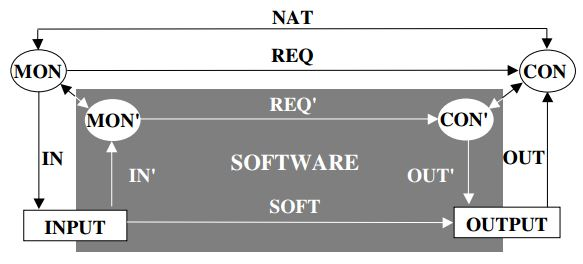
\includegraphics[scale=0.6] {images/FourVarExtn.jpg}
    \caption{Extension of Four Variable Model}
    \label{fig:extn-four-var}
 \end{figure}

To address this concern for the software, Miller et al extended the four variable model, as shown in Figure~\ref{fig:extn-four-var}. They recreate virtual versions of the variables $mon'$ and $con'$ that differ from the original $mon$ and $con$ in terms of value and timing introduced when sensing and setting the input and output variables. Using these virtual variables, they ``stretch'' the $SOF$ (software) relationship into $IN'$, $REQ'$, and $OUT'$. The $IN'$ and $OUT'$ represents the specification of hardware drivers that were previously part of the $SOF$. With this change, they propose a mere recapture of each function in $REQ$ to $REQ'$ using corresponding variables. They assert that this makes the tracing of the requirements REQ to the software ($REQ'$) direct and straightforward. While this approach superficially seems indisputable and makes the task of decomposition simpler, in our experience, we found that this approach could result in inaccurately specified and verified component requirements.

The overall system requirements especially for complex control systems such as GPCA are typically captured in such a way to accommodate certain degree of inaccuracies and imperfections. For example, lets consider a system level requirement:

\begin{quotation}
\emph{``In basal mode, the system shall infuse the drug at a flow rate within $BasalFr$ $\pm t$\% tolerance''}
\end{quotation}

The tolerance (t) in this requirement was included to accommodate inaccuracies of the physical components that is going to be used in the GPCA. Mathematically, this requirement is a relation, since the flow rate (output) is allowed to have range of values. When we decomposed the GPCA into various components and tried to allocate requirements to the software (one of the components of GPCA), we were tempted to formalize requirements for verification such that it mirrors the system requirement but in terms of inputs and outputs of the software, such as:
\\\\
\footnotesize{\texttt{
(Mode = basal) $\Rightarrow$\\
\textcolor{white}{------}FlowRate $\leq$ (1 + t/100) $\ast$ (BasalFr) and \\
\textcolor{white}{------}FlowRate $\geq$ (1 - t/100) $\ast$ (BasalFr)\\
}}
\normalsize{}\\
While the above formulation appears to be correct and mirrors the system level requirement, the tolerance part was not intended to be allocated to the software. When we model checked this requirement it was successfully verified since the software indeed satisfied, but in an unintended fashion. In reality, the software's output is deterministic and there was no need for the tolerance, hence the consequent in the formalization was supposed to be \texttt{(FlowRate $=$ BasalFr)}. That is, mathematically the requirement of the software is a function as opposed to the system level requirement that is a relation. %In our opinion, failing to understand these differences in mathematical formulation leads to inaccurate understanding of formal verification.

While superficially this doesn't appear to be a problem, an indepth analysis revels that this leads to a situation in which we could prove the system level requirements with just the software requirements. The way we formalized the software requirement is not only an over approximation of the capabilities of the software but also masks the other component requirements. Unfortunately, this was not apparently visible until we started analysing how the software requirements realizes the system level requirements.

\subsubsection {Solution : Traceability Argument}

To address this issue, we developed a \emph{traceability argument} between requirements at adjacent levels in the hierarchy. Unlike the traditional traceability in which each parent level requirement is traced to its corresponding child requirement, we documented an argument of traceability that captures how child component requirements contribute to satisfying the system level requirement. This sort of assurance argument, that is inspired from Hammond's work on documenting justification for design decisions~\cite{Hammond01:WiW}, helped us understand the role of each component in satisfying the system requirement. In fact, by documenting the \emph{traceability argument} we were able to identify 8 incorrectly formalized component requirements of the GPCA. Further, this argument also helped us identify the component requirements that did not contribute to satisfying any of its parent level requirement. In sum, the traceability argument clarified the role and relevance of each requirement in satisfying its parent requirement, that in-turn helped identify the formalization errors in capturing them. While documenting this form of argument is not difficult when it is done at the time of requirements allocation, establishing this traceability after all requirements are allocated might be laborious. To address that concern, we are currently working towards building an automated traceability capability in the AGREE tool. This capability would automatically identify for every system requirement (parent level) the set of child component requirements that contributed to satisfying it. The task left for the developer is only to document the justification for the traceability.

\subsection{Tool Fallibilities}

Although we used sophisticated tools with advanced capabilities such as consistency checks, cursory knowledge about how the tools perform such checks lead us to successfully verify inconsistent requirements. The tool we used -- AGREE -- had capability to check consistency of requirements in addition to verifying them that detects logical contradictions among requirements. The intent of performing such checks is to identify if the verification was trivially successful due to presence of inconsistent requirements. While the tool declared that all the GPCA requirements are consistent, our tool expert during the manually inspection phase found that there were several self-inconsistent requirements. To our surprise, those inconsistencies were not reported by the tool. This was primarily because we did not have full knowledge of the tool settings associated with that check.

Lets us illustrate the problem with an concrete example. To formalize certain requirements for GPCA we had to specify counters to keep track of duration of internal conditions or occurrence of certain actions. For example, consider a requirement to notify the clinician when the patient requests more than a certain number of boluses. To formalize this requirement we had to count the number of requests received \texttt{(PatientRequest)} by the system. Hence, we declared an integer variable \texttt{(boluscnt)}, whose initial value was 0 and then gets incremented whenever a \texttt{PatientRequest} is received by the system, as shown below. The formal language shown below is based on Property Specification Language (PSL) [16] and defines a Lustre language
[11] “flavor” for the PSL expressions. Lustre is a synchronous dataflow language that describes the behavior of a system through a set of equations, and it can be viewed as a textual analogue to Simulink block diagrams. In this notation, it is possible to define constants, local variables and reusable fragments of temporal logic (called properties). Additionally, we can describe stateful relationships between variables using
the `pre' expression, which provides the value of a variable from the previous step of execution of the system. In the following formalization, "->" is used to capture the sequence of value computations for a variable. For example "0 -> 5" means the initial value is 0 and all the subsequent values are 5. We encoded the GPCA requirements using this notation.

$$ \texttt{boluscnt:int = 0 -> boluscnt + PatientRequest} $$

While the tool successfully verified the above requirement involving the \texttt{boluscnt} variable, during manual inspection our tool expert pointed out this statement was internally inconsistent. The inconsistency was due to the usage of \texttt{boluscnt} in both the right and left side of the equation. According to the tool, the value for \texttt{boluscnt} always refers to its value in the current time step, whereas we actually intended to refer to the value in the previous time step in the right side of the expression. The incorrect formulation had caused a circular dependency in assigning values for \texttt{boluscnt} variable, that made this expression and the requirement involving this variable inconsistent and trivially satisfied. In the GPCA, we identified 20 such inconsistent formalizations in both system and component levels. To fix this issue, we used AGREE's operator \emph{``pre"}, to refer to the value of a variable in the previous step as shown below.

$$ \texttt{boluscnt:int = 0 -> pre(boluscnt) + PatientRequest} $$

While adding \emph{``pre"} fixed this specific type of inconsistency, our concern was that the tool's consistency checker did not identify this problem. After discussing with the tool developers, we found that the tool was set up by default to check for consistency only in the initial time step (first step of execution). This was not a bug in the tool, rather an intensional default setting to optimize the performance of the tool. According to the tool developers, most inconsistencies can be found in the first step and this was an exceptional condition. Since the \texttt{boluscnt} equation was inconsistent only after the initial step (its initial value was 0), the consistency checker did not report the problem. 

In our opinion, this situation is not limited to this specific example or tool but generalizable for all model checking tools and techniques. The root cause of this problem is not just our cursory knowledge of the tools, but also the lack of adequate details of the task displayed by the tool. %To mitigate this problem, in addition to validating the formalization with domain and tool experts, an indepth understanding of the tool settings that performs such checks and validations, rather than blindly trusting the results from the tool.


%Hence, when the tool developers
%
%Although the tool was sophisticated enough to allow this default setting to be changed, the real problem was our cursory knowledge about the tool and the fact that it was not obvious from the tool results. While we fixed this issue by both changing the formalization as well as enhancing the tool to display the number of time steps for consistency check, the risk of specifying such inconsistent requirements could only be avoided if we had through understanding of the tool.
%
%

\subsection{Matching Tool Boundaries}

While it is ideal to use a tool/technique to verify the entire system's requirements, in practice it is inevitable to avoid the use of multiple tools for scalability concerns and different verification needs. One of the well known problems associated with using multiple tools is matching the sematic differences between them. In an earlier effort, in which we semiformally mapped abstraction differences between infusion pump requirements formalized and captured as timed automata and AGREE notation, we identified semantic errors in the the mapping, in particular differences in the way time is handled in the notations. We fixed those issues by defining a formal semantics~\cite{whalen2015hierarchical} to rigorously map the models and their requirements. However, we found that even when tools with ``same" semantics were used rigorously maintaining the relationship between them in the long run is challenge.

In GPCA, we used a combination of two tools to cope with scalability of verification. We used AGREE to model the system architecture and verify the decomposition of system requirements into component requirements. Subsequently, we also developed detailed behavioral models for each component in Simulink and verified if the component requirements verified in AGREE are indeed satisfied by the respective component's behavioral model using Simulink Design Verifier (SDV). The advantage of this tool combination in addition to being scalable is that the semantics of the notation used in AGREE and SDV (Embedded Matlab) to specify requirements are comparable. Hence, we presumed that the translation of requirements between AGREE and Simulink notations can be done in a error free manner.

While a majority of the requirements were correctly recaptured between the notations some requirements were incorrectly recaptured that, unfortunately, was not easy to detect. We identified two such issues - transcription errors and requirement management issues. The transcription errors occurred in the process of manually recapturing requirements. When recapturing some requirements we unknowingly changed the operators. In GPCA, we translated the following requirements that were proved in Simulink into AGREE as :

\scriptsize{
\begin{verbatim}
Properties in Embedded Matlab:
-----------------------------
sldv.prove(
    implies(SystemOn and AirInLine),(FlowRate <= MedFlow))
sldv.prove(
    implies(SystemOn and EmptyReservoir),(FlowRate <= LowFlow))
    
Property in AGREE:
----------------------------
guarantee "Property1": 
    (SystemOn && AirInLine) => (FlowRate $=$ MedFlow)
guarantee "Property2":
    (SystemOn && EmptyReservoir) => (FlowRate $=$ LowFlow)    
\end{verbatim}
}
\normalsize{}

It was not possible to dismiss this error as a mere typo, since it demonstrates the potential for occurrence of such issues. Unfortunately, this error was not visible until we checked for feasibility using a recent enhancement of AGREE's tool called \emph{realizability}. Intuitively, realizability checks if there is exists an output of the system for every input that satisfies the requirements. In the above case, the realizability check identified a counterexample in which both AirInLine and EmptyReservoir\footnote{AirInLine indicates a hazard in which air bubble(s) are detected in the infusion tubing and EmptyReservoir is a hazard that indicates that the drug reservoir does not have sufficient drug to infuse}. While this feature was not intended to identify the recapture errors, coincidentally we were able to identify this issue. After the found this errors, on manual inspection we identified 6 such transcription issues and corrected them. 

Another issue, that we believe is more common, is maintaining the synchrony between the requirements in both tools. After we proved requirements in AGREE, when we recaptured it for verification using SDV, at times we had to slightly change the way requirements were formalized, such that it is verifiable in the behavioral Simulink. However, such changes were sometimes missed to be changed and reverified in AGREE - another human error that caused mismatch between the requirements. Although we were diligent in recapturing the requirements between the tools, human errors and negligence was unavoidable. For the GPCA, we did additional manual inspections to verify the synchrony. However, in our opinion, a lack of rigours process and/or automation to translate and check for synchrony is the root cause of this problem. %to avoid such issues. Infact, our recommendation to engineers performing such tasks is to ensure there is either a strict process or automation to avoid such issues.


%\section{Recommendations}
\label{sec:recommendations}

On analysing the root causes of each of the challenges, we assert that to realize the benefits of using formal methods to verify requirements we need adapt both the requirements engineering activities to support formal methods as well as the formal techniques to recognize common requirement verification concerns. In this section, we elaborate on how we addressed the first two challenges by changing requirements engineering process and the other two challenges by changing and enhancing the formal tools.

\subsection {Solution To Challenge 1: Structuring Requirements}

To systematically identify the context of each requirement and its dependencies with other requirements, we hierarchically restructured the GPCA requirement document as shown in Figure~\ref{fig:gpca-requirements}, that not only simplified the formalization process also helped understand the system in a conceptually clear way. The system behaviors of most control systems are typically captured by grouping them in terms of \emph{modes} - a logical way to describe a set of system behaviours. In a complex system, there could be many modes that could either be mutually exclusive (only one mode can be active at a time) or orthogonal (multiple modes can be active at a time). By grouping the modes based on their common and exclusive behaviours as well as their interactions, we hierarchically organized them that helped systematically documenting, formalizing and verifying the requirements.

 \begin{figure}[h!]
    \centering
    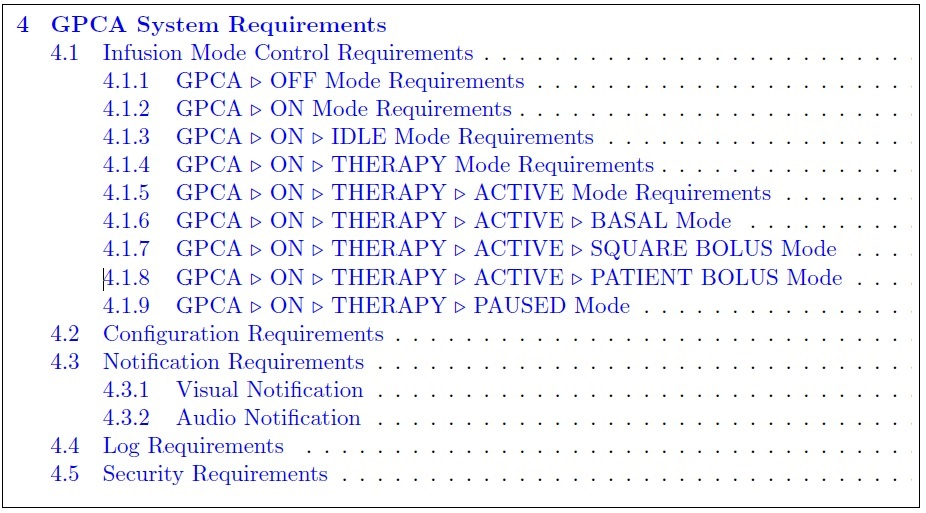
\includegraphics[width=\columnwidth]{images/structuring.jpg}
    \caption{GPCA System Requirements Structuring}
    \label{fig:gpca-requirements}
 \end{figure}

In the GPCA, there were three main orthogonal groups of modes - infusion, configuration and notification modes. Within each orthogonal group, there were a set of modes that were mutually exclusive to each other such as basal, intermittent and patient bolus modes within infusion mode group. Similarly, the notification group had 18 requirements that we further categorized based on its severity level (Levels 4 to 1). When we analysed the requirements, we understood that there were many requirements that were common to the exclusive modes among an orthogonal group, as well as requirements that were common to all the three orthogonal mode groups. We leveraged this pattern of modal requirements to organize requirement statements within the document in an hierarchial fashion. In this structuring, at the top most level we placed requirements that were common to the entire system. At the next level, we placed the mode groups that were orthogonal to each other. Within each orthogonal mode group, we again followed the hierarchical structure to organize their requirements. For clarity purposes, within a mode group we grouped requirements hierarchically based on their behaviours and named it as a new mode (although it was not explicitly mentioned by the stakeholders). For example, we placed all the requirements that were common among the basal and boluses infusions in a parent mode called \emph{Therapy} mode and made the basal and bolus its child modes with its own set of special requirements. For additional clarity on understanding the mutual exclusivity among modal behaviours, we documented requirements using a tabular notation. An example of the tabular format we used for the notification requirements is shown in Figure~\ref{fig:gpca-alarm}. Although we came across a couple of requirements that had minor variations to be grouped, this structuring helped identify those differences and we were able to clearly negotiate with our domain experts on appropriately categorizing them. 

 \begin{figure}[h!]
    \centering
    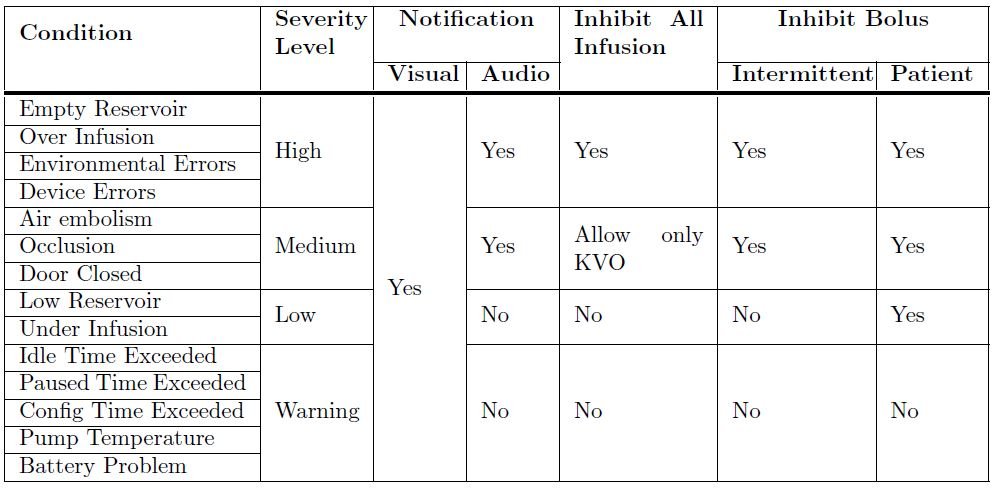
\includegraphics[width=\columnwidth]{images/alarm.jpg}
    \caption{Notification Requirements Table}
    \label{fig:gpca-alarm}
 \end{figure}


This structuring greatly helped in systematically determining the context of each requirement while formalizing it. It provided enough information about the orthogonality and exclusivity among the modes. For instance, by examining the requirements hierarchically from the top level, we were able to precisely identify and formalize the context of the patient bolus infusion requirement and the notification requirements that were discussed in Section 3.1. While such hierarchical structuring is common among modeling community, it has not been widely used to document requirements in the requirements engineering community. We believe that using such a strategy not only helps reducing the effort for formalizing requirements, but also provides the intellectual clarity to understand the system behaviours.
%%
%%such as the operating condition of the system (whether the system is ON/OFF), clinician's inputs that have influence over the entire system and the various levels of exceptional conditions documented in the alarm hierarchy requirements as shown below.
%%Infact, in some cases it helped us identify and raise the right questions to discover incomplete requirements within a hierarchical level. Overall this structuring allowed the process of formalization straightforward, that otherwise would have been an ardours trial and error approach.  %Another significant benefit of this structuring is the clarity it provides in documenting the mode transition requirements within infusion modes - descriptions about how and when transitions between those modes occur. We documented the requirements on transitions between the three modes within therapy mode, its immediate parent mode. This strategy allowed us to systematically formalize and verify the mode transition requirements -- a common source of problem in modal systems.
%%For example, the formalized requirements for patient bolus infusion was:
%\\\\
%\footnotesize{\texttt{
%SystemOn~and~not(ClinicianInhibits) and not(level2alarms and level3alams and level4alarms) and \\ \textcolor{white}{---}~and~(PatientRequest)~$\Rightarrow$ \\
%\textcolor{white}{--------}FlowRate~=~PatientFr}}
%\\\normalsize{}\\
%
%Similarly, formalizing the alarm requirements to verify them individually also became straightforward. Grouping the exceptional conditions and its associated actions in the requirements document eased the process of formalizing the requirements. We used variables (or macros) to capture the conditions that cause that alarm level and the desired actions, to avoid repetition in definitions. It then became systematic and straightforward to individually check a requirement. For example, in the GPCA there were 3 exceptional conditions that we categorized as medium level alarms, namely air in line (sensor input indicating air in infusion tube), occlusion (sensor input indicating blockage in infusion tube) and door open (sensor input indicating drug reservoir enclosure is opened). To check the door open requirement exclusively, we systematically excluded the all higher priority level alarm (HiLevelAlarm is a logical disjunction of all conditions within the highest severity level) and the other conditions in its peer level, as shown below :
%\\\\
%\footnotesize{\texttt{SystemOn and not(HiLevelAlarm) and \\
%\textcolor{white}{----}not(AirInLine) and not(Occlusion) and \\ \textcolor{white}{------}(DoorOpen)$\Rightarrow$\\
%\textcolor{white}{--------} MedLevelAlarmActions}}
%\\\normalsize{}
%


\subsection {Solution For Challenge 2: Richer Traceability}

When we identified the issue of formalizing the flow down requirements incorrectly, we started documenting a \emph{traceability argument} between requirements at adjacent levels in the hierarchy. Unlike the traditional traceability document, in which each parent level requirement is traced to its corresponding child requirement, we additionally documented an argument (a semiformal statement) explaining how the child requirement contributes to satisfying the system level requirement. This sort of assurance argument, that is inspired from Hammond's work on documenting justification for design decisions~\cite{Hammond01:WiW}, helped us understand the role of each component in satisfying the system requirement. In fact, by documenting the \emph{traceability argument} we were able to identify 8 incorrectly formalized component requirements of the GPCA. Further, this argument also helped us identify the component requirements that did not contribute to satisfying any of its parent level requirement. In sum, the traceability argument clarified the role and relevance of each requirement in satisfying its parent requirement, that in-turn helped identify the formalization errors in capturing them. To enhance the rigour of this approach, we are currently working towards building an automated traceability capability in the AGREE tool.

%
% \begin{figure}[h!]
%    \centering
%    \includegraphics[width=\columnwidth]{images/traceability.jpg}
%    \caption{Snippet from Richer Traceability Document}
%    \label{fig:gpca-alarm}
% \end{figure}


\subsection {Solution For Challenge 3: Sanity Checks and Fallibility Detection}

We believe that the root cause of the AGREE tool not identifying the consistency issues in the formalized requirements was not the tool's default setting, but the fact that it was not apparent in the results. Hence, to address the issue from the tool side we requested the tool developers to provide elaborate messages of certain key configurations when using the features, that play a key role in determining their correctness. After that change, AGREE now displays the depth of consistency check along with the results. While such a change may not be possible with every tool and feature we use, we strongly recommend the engineers to delve deep into the details and configuration of tool to precisely understand the results, especially when there is limited information provided by the tool along with the results. Additionally, this error motivated the tool developers to enhance the AGREE tool to check for \emph{vacuity}. We believe with vacuity checking we could effectively identify some of these issues. 

\subsection {Solution For Challenge 4: Automating Verifiers}

To address the transcription errors for GPCA, we first strengthened the process of verifying the translation using code inspection by a different developers. This inspection was effective in identifying errors, but was time consuming. In the long run, to maintain the synchrony between the requirements in both the tools was challenging. This challenge became the motivation for another team who are currently developing an automated translator that recaptures properties from AGREE tool notation to Embedded Matlab notation and vice-versa. While we are not actively involved in the development of the automation, we are currently verifying and validating their work using the GPCA's manual translation. While code inspections were effective, automated translators significantly reduced the overall time in the overall process. 
\section{Discussion and Conclusion}
\label{sec:conclusion}

In this paper, we elaborated on the challenges encountered while adopting formal methods for engineering requirements of a complex medical device system.


\iffalse
\section{Infusion Pump - Case Example}
\section{Formalizing Requirements}

using the Specific challenges - I would like to explain our approach right after each challenge.

1a. Formalizing Alarm requirements - Individually checking each alarm effect - same functionality but different priority. - no higher level alarm is active.

\vspace{2mm}

1b. Formalizing Alarm requirements - Notification Requirements - Priority in notification.

\vspace{2mm}

2. Formalizing Infusion manager requirements - Functional requirements - Requires alarms and other conditions to be specified. - orthogonal mode concerns.

\vspace{2mm}
3. Formalizing Configuration manager requirements - Requires sequence of actions to be formalized.

\section{Tracing Requirements}

About traceability with justification - informal traceability between system requirements and software requirements. Scope mapping issue - parts of system requirements map to parts of software requirements. How to map them - the justification serves as a link.

\vspace{2mm}

explain how we assume just one component implements the system requirements - but other component requirement are necessary to satisfy the requirements. Our semi-automatic approach to identify min set of component requirements.

\vspace{2mm}

Explain how we tried to reuse the system level requirements to software. Even without hardware requirements the system requirements were satisfied. Also Problems if we treat both system and software requirements as functional.

\section{Pitfalls of Formal Verifications}

In this section, we describe how tools produced misleading/false positive results.

\vspace{2mm}
1. using output variables to formalize requirements. We need to include inputs that capture output's correctness. for example:

output 1 => ouput 2
is not good. we should have some clarity on what that outout1 means with respect to inputs.

\vspace{2mm}

2. how to access what have we covered - we could describe how we formalized notification requirements -

a or b or c => message 1 or 2 or 3

!a => !1...

We havent specified what happens if 2 and 3 happens at the same time.

\vspace{2mm}
3. failed Consistency and realizability checking - The case we formalized it using circular dependencies internally. But the consistency and realizability checks failed.
\fi

%\vspace{0.5in}
\bibliographystyle{plain}
\bibliography{crisys}
%\balancecolumns

\end{document} 